%!TEX root = ./WTG.tex

\section{Erstes Kapitel}

\begin{definition}[Netzwerk] 
	\label{def:Netzwerk}
	\marginnote{Mit anderen Worten: Ein Netzwerk ist ein positiv gewichteter Graph.} 
	Ein Netzwerk $G = (V,E,c)$ ist ein Graph $\enb{V,E}$ mit entweder gerichteten oder ungerichteten Kanten, d.h.
	\begin{align}
		E \subseteq \set{\enb{x,y} \given x,y \in V} && \text{beziehungsweise} && E \subseteq \set{\set{x,y} \given x,y \in V},
	\end{align}
	zusammen mit einer Gewichtsfunktion $c:E \to \Real^+$.
\end{definition}

Ist nun $\enb{X_n}_n$ eine Irrfahrt auf $\enb{V,E}$ mit Übergangswahrscheinlichkeiten $P = \enb{p_{xy}}$, dann wollen wir daraus ein Netzwerk konstruieren. Dazu nehmen wir an, dass die Irrfahrt \emph{reversibel} bezüglich eines Maßes $\pi$ auf $V$ ist.
\begin{gather}
	\pi\enb{x}p_{xy} = \pi\enb{y} p_{yx}
\end{gather}
Dabei muss $\pi$ kein Wahrscheinlichkeitsmaß sein.

\begin{bemerkung}
	Das Maß $\pi$ ist stationär für die Markovkette.
\end{bemerkung}
\begin{beweis}
	Zu zeigen: $\pi \cdot \p = \pi$. 
	\begin{gather}
		\marginnote{$y\sim x:=$ alle $y$ die zu $x$ benachbart sind.}
		\pi\enb{x} = \pi\enb{x} \sum\limits_{y \sim x} p_{xy} = \sum\limits_{y \sim x} \pi(x)p_{xy} = \sum\limits_{y\sim x} \pi(y)p_{yx}.
	\end{gather}
\end{beweis}
Wählt man nun $c(x,y):=\pi(x)p_{xy}$ so gilt $c(x,y)=\pi(x)p_{xy} = \pi(y)p_{yx} =  c(y,x)$.
Das Kantengewicht ist also unabhängig von der Orientierung der Kante. Zusammenfassend haben wir nun festgestellt, dass eine reversible Irrfahrt bezüglich $\pi$ auf $(V,E)$ ein Netzwerk mit Kantengewicht $c(x,y) = \pi(x)\p_{xy} = c(y,x)$ induziert.

Umgekehrt existiert es zu einem gegebenen Netzwerk $(V,E,c)$ eine Irrfahrt auf $(V,E)$, mit $p_{xy} \approx c(x,y)$. Genauer: 
\begin{gather}	
p_{xy} = \frac{1}{\sum\limits_{z \sim x}} \cdot c(x,y) = \frac{c(x,y)}{\pi(x)}.
\end{gather}
Gilt $c(x,y) = c(y,x)$ für alle $x,y$, so ist die Irrfahrt bezüglich $\pi$ reversibel, denn 
\begin{gather}
	\pi(x)p_{xy} = c(x,y) = c(y,x) = \pi(y)p_{yx} 
\end{gather}

\begin{beispiel}[Gambler's Run]
	\label{bsp:GamblersRun}
	Sei $X_n$ eine Irrfahrt auf $\set{0, \dots, n}$ und	
	\begin{gather}
		\prop{X_n = i+1 \given X_{n-1} = i} = p = 1 - \prop{X_n = i-1 \given X_{n-1} = i}.
	\end{gather}
	Wie kommt man nun auf die Kantengewichte?
	\begin{gather}
		\prop{X_{n+1} = i+1 \given X_n = i} = \frac{c(i,i+1)}{c(i,i+1)+c(i,i-1)} = \frac{\enb{\frac{p}{q}}^i}{\enb{\frac{p}{q}}^i + \enb{\frac{p}{q}}^{i-1}} = \frac{\frac{p}{q}}{\frac{p}{q} +1} = p
	\end{gather}
	Sei nun $A,Z \subseteq V, A \cap Z = \emptyset$. Was ist nun $\prop{\tau_A < \tau_Z}[][x]?$ (Wobei $\tau_1$ die erste Treffzeit der Menge $A$ ist und $\p_x$ die Wahrscheinlichkeit, bei Start in $x$). Sei $F(x) = \prop{\tau_A < \tau_Z}[][x]$, dann ist $F|_A = 1$ und $F|_Z = 0$. Ist $x \notin A \cup Z$, dann ist $\set{x,y} \in E$ 
	\begin{equation}
		F(x) = \sum\limits_{y \sim x} p_{xy} F(y) = \frac{1}{\pi(x)} \sum\limits_{y \sim x} c(x,y)F(y) \tag{*} \label{eqn:GamblersRun}
	\end{equation}
	Im einfachsten Fall (Simple Random Walk) ist $c(x,y) = 1$ und $\pi(x) = \deg(x)$ \marginnote{$\deg(x)$ ist der Grad von $x$} und wir haben
	\begin{equation}
		F(x) = \frac{1}{\deg(x)} \sum\limits_{y \sim x} F(y),
	\end{equation}
	also ist $F(x)$ der Mittelwert all seiner Nachbarn. 
\end{beispiel}

\begin{definition}	
	Eine Funktion $F$, welche \eqref{eqn:GamblersRun} erfüllt, heißt harmonisch in $x$ bezüglich der Gewichte $c$. Ist $F$ harmonisch für alle $x \in V$ so heißt es nur harmonisch.
\end{definition}
Harmonische Funktionen erfüllen einige nützliche Prinzipien, Dazu sei für $W \subseteq V$
\begin{align}
	\delta W := \set{y \notin W \given \exists x \in W: y \sim x} && \overline{W} = W \cup \delta W
\end{align}
\begin{satz}[Maximumsprinzip]
	Sei $G(V,E,c)$ endlich oder unendlich und $H = (V(H),E(H),c)$ ein endliches zusammenhängendes Teilnetzwerk. Sei $f: V \to \RR$ harmonisch auf $H$. Falls dann gilt
	\begin{align}
		\max\limits_{x \in V(H)} f(x) = \sup\limits_G f
	\end{align}
	so gilt auf $V(H)$:
	\begin{align}
		f \equiv \sup f 
	\end{align}
\end{satz}
\begin{beweis}
	Sei $K := \set{f(x) = \sup f \given x \in V}$. Ist $x \in K \cap V(H)$, so gilt
	\begin{equation}
		\sup f = f(x) = \frac{1}{\pi(x)} \sum\limits_{y \sim x} c(x,y) f(y) \Rightarrow f(y) = f(x)
	\end{equation}
	für alle $y \sim x$. Das heißt, mit $x \in K$ sind auch alle $y \sim x$ in $K$. Da $V(H)$ endlich und zusammenhängend ist, kann man dies iterieren und kommt so bis $V(H) \cup \delta V(H) = \overline{V}(H)$.
\end{beweis}

\begin{korollar}[Eindeutigkeitsprinzip]
	\label{kor:Eindeutigkeitsprinzip}
	Sei $G = (V,E,c)$ beliebig, $W \subseteq V$ endlich. Falls $f,g: V \to \RR$ harmonisch auf $W$ sind, so folgt
	\begin{align}
		f|_{V\backslash W} = g|_{V\backslash W} \Rightarrow f = g
	\end{align}
\end{korollar}
\begin{beweis}
	Die Funktion $h = f - g$ ist harmonisch auf $W$ und $h=0$ auf $V\backslash W$. Wähle $x \in W$, sodass $h(x) > 0$ maximal ist. Wähle die Zusammenhangskomponente $W_0$ in der $x$ liegt. Dann ist $h \equiv h(x)$ auf $W_0 \cup \delta W_0$. Aber $\delta W \subseteq V \backslash W$ und dort ist $h(x) = 0 \lightning \Rightarrow h \leq 0$ überall. 
	
	Das gleiche stimmt für $\overline{h} = g-f \leq 0$.
\end{beweis}

\begin{korollar}
	\label{kor:1-7}
	Sei $V$ endlich, $A,Z \subseteq V, v \cap Z = \emptyset$. $G \colon V \to \Real$ erfüllen $G|_A = 1, G|_Z \equiv 0$ $G$ harmonisch auf $V \backslash (A \cap Z)$. Dann ist $G(x) = F(x) = \prop{\tau_A < \tau_Z}[][x]$
\end{korollar}
\begin{beweis}
	Folgt aus dem Eindeutigkeitsprinzip, wenn man $W = V\backslash (A \cap Z)$
\end{beweis}

\begin{satz}[Existenzprinzip]
	Sei $V$ endlich oder unendlich, $G = (V,E,c)$. Sei $W \nsubseteq V$ und $f_0 \colon V_0 \backslash W \to \Real$ beschränkt. Dann gibt es eine Funktion $f \colon V \to \Real$, sodass $f|_(v \backslash W) = f_0$ und $f|_W$ harmonisch.
\end{satz}

\begin{beweis}
	Starte die Netzwerk-Irrfahrt $(X_n)$, d.h. die deren Übergangswahrscheinlichkeiten durch $c(x,y)$ bestimmt sind. Sei $X$ die ZV, die angibt, wann $(X_n)$ die Menge $V \backslash W$ trifft, falls dies überhaupt der Fall ist. Sei
	\begin{gather}
		Y = 
		\begin{cases}
			f_0(X), & \text{falls} (X_n) \text{ die Menge } V \backslash W \text{ trifft } \\
			0, & \text{ sonst}
		\end{cases}
	\end{gather}
	Behauptung: $\EW{Y}$ ist eine harmonische Fortsetzung von $f_0$
\end{beweis}
\begin{uebung}
	Berechnen Sie im Gambler's Run die Wahrscheinlichkeit links oder rechts anzuschlagen, sowie die erwartete Treffzeit.
	\begin{figure}[htbp]
		\begin{minipage}{0.4\textwidth}
			\begin{tikzpicture}[scale = 0.8]
				\draw(0,0) to (7,0);
				\draw(0,3pt) to (0,-3pt) node[below] {0};
				\draw(7,3pt) to (7,-3pt) node[below] {n};
				\draw(3,3pt) to (3,-3pt);
				\draw [->, bend angle=45, bend right] (3,0) to (2,0);
				\draw [->, bend angle=45, bend left] (3,0) to (4,0);
				\draw node at(2.5,0.35) {$p-1$};
				\draw node at(3.5,0.35) {$p$};
			\end{tikzpicture}	
		\end{minipage} 
		\hfill
		\begin{minipage}{0.4\textwidth}
			\centering
			$p_X = p \cdot p_{X+1} + (1-p) p_{X-1} $
		\end{minipage}
	\end{figure}
\end{uebung}
Wir bertrachten jetzt ein Netzwerk als ein elektrisches Netzwerk, d.h. $c(x,y)$ sei die Leitfähigkeit und $\frac{1}{c(x,y)} = r(x,y)$ sei der Widerstand der Kante $(x,y)$. Wir legen in einem $a$ eine Spannung $v(a)$ an und leiten einen Strom $i$ durch das Netztwer, das in $Z \subseteq V$ abfließt ($v(z) = 0, \forall z \in Z$). Es gelten die klassischen Regeln der Elektrizitätslehre:

\begin{regel}[Ohmsches Gesetz]
	\label{regel:ohm}
	\begin{align}
		\forall x\sim y: v(x)-v(y) = i(x,y) \cdot r(x,y) = \frac{i(x,y)}{c(x,y)}
	\end{align}
\end{regel}

\begin{regel}[Kirchhoffsches Gesetz]
	\label{regel:kirch}
	\begin{align}
		\forall x \notin \set{a} \cup Z: \sum\limits_{y \sim x} i(x,y) = 0
	\end{align}
\end{regel}

Aus diesen Regeln lassen sich einige Konsequenzen ableiten:
\begin{itemize}
	\item da $c(x,y) = c(y,x) \Rightarrow i(x,y) = c(x,y)\big(v(x) -v(y)\big) = -c(x,y)\big(v(y)- v(x)\big) = - i(y,x)$
	\item da $c(x,y) > 0 \Rightarrow \Big({i(x,y) > 0 \Leftrightarrow v(x) > v(y)}\Big)$
	\item ist $x \notin A \cup Z$, so gilt nach \ref{regel:kirch} 
		\begin{align}
			0 = \sum\limits_{y \sim x} i(x,y) = \sum\limits_{y \sim x} \big[v(x)-v(y)\big]c(x,y)
		\end{align}
		Und wegen $c(x,y) = p_{xy} \cdot \pi(x)$, sowie im darauffolgenden Schritt $\sum\limits_{y \sim x} p_{xy} = 1$, folgt
		\begin{align}
			\Rightarrow \sum\limits_{y\sim x} v(y)c(x,y) = v(x)\pi(x) \sum\limits_{y \sim x} p_{xy} \\
			\Rightarrow v(x) = \frac{1}{\pi(x)} \sum\limits_{y \sim x} v(y) c(x,y)
		\end{align}
\end{itemize}
Also folgt aus \ref{regel:ohm} und \ref{regel:kirch}, dass $v$ harmonisch ist. Wenn also $V$ endlich ist, $V|_A = 1$ und $V|_Z \equiv 0$ ist, so folgt mit \ref{kor:1-7} $v(x) = \prop{\tau_A < \tau_Z}[][x]$

\begin{korollar}[Kirchhoffsche Maschenregel]
	Sei $x_1 \sim x_2 \sim \dots \sim x_n \sim x_1$ ein Kreis. Dann gilt 
	\begin{align}
		\sum\limits_{j=1}^{n}i(x_j,x_{j+1})r(x_j,x_{j+1}) = \sum\limits_{0}^{n}v(x_{j+1}) - v(x_j) = 0
	\end{align}
\end{korollar}

\section{Irrfahrte auf elektrischen Netzwerken}
Zunächst sei $G(V,E,c)$ nun immer ein endliches Netzwerk. Sei $a \in V$ und $Z \subseteq V$. Wir fragen uns nach der Wahrscheinlichkeit mit der Irrfahrt vom Startpunkt $a$ $Z$ zu erreichen, bevor wir wieder nach $a$ zurückkommen, also $\prop{a \to Z} = \prop{\tau_Z < \tau_{\set{a}}}[][a]$. Das wird insbesondere interessant, wenn $G$ unendlich, $G_n$ unendlich mit $G_n \uparrow G$ und  $Z = \delta G_n$ und $a=0$.

Dann fragt man sich offenbar nach der Wahrscheinlichkeit gegebenenfalls sehr weit von Ursprung entfernte Mengen $Z$ zu erreichen, bevor man $0$ wieder sieht. Das ist nichts anderes als Transienz. Wir wollen $\propE{a \to Z}[][a]$ studieren. Legen wir an $a$ eine Spannung $v(a)$ an und lassen $v(z) = 0, \forall z \in Z$ sein, dann ist $v$ auf $V \backslash(\set{a}\cup Z)$ harmonisch, aber auch $\propE{\tau_A < \tau_Z}[][x]$. Wegen des Eindeutigkeitsprinzips (\ref{kor:Eindeutigkeitsprinzip}) unterscheiden sich beide nun um $\frac{1}{v(a)}$, d.h. $\prop{\tau_a < \tau_Z}[][x] = \frac{v(x)}{v(a)}$. Also
\begin{align}
	\prop{a \to Z} = \sum\limits_{x}p_{ax} \Big(1-\prop{\tau_a \tau_Z}[][x] \Big) &= \sum\limits_{x}\frac{c(a,x)}{\pi(a)}\enb{1-\frac{v(x)}{v(a)}} \\
	&= \frac{1}{\pi(a)v(a)}\sum\limits_{x}c(a,x)\big(v(a)-v(x) \big) \\
	&= \frac{1}{\pi(a)v(a)}\sum\limits_{x}i(a,x)
\end{align}

\begin{align}
	\Rightarrow v(a) = \frac{\sum\limits_{x}i(a,x)}{\pi(a)\prop{a \to Z}}
\end{align}
Da $v(z) = 0$ auf $Z$, hat das Ganze wieder die Gestalt des Ohmschen Gesetztes \ref{regel:ohm}, wenn man den Nenner als Leitfähigkeit interpretiert. Tatsächlich heißt $\pi(a)\prop{a \to Z}$ die effektive Leitfähigkeit von $a$ nach $Z$ und wir schreiben
\begin{align} 
	\leit{a \leftrightarrow Z} = \mathcal{C}_{eff}  = \leit{a\leftrightarrow Z,G}
\end{align}
Den effektive Widerstand ist somit 
\begin{align}
	\frac{1}{\leit{a \to Z}} = R(a \leftrightarrow Z)
\end{align}
Offenbar ist $\prop{a\to Z} = \frac{\leit{a \leftrightarrow Z}}{\pi(a)}$. Das hilft allerdings nur, wenn $\leit{a \leftrightarrow Z}$ gut ausrechnen kann. 

Sei nun $X$ die Anzahl der Besuche von $X_n$ in $a$ bevor $X_n$ in $Z$ absorbiert wird. Wir betrachten zunächst den Start in $a$. Sei 
\begin{align}
	X \sim Geo(p) mit p= \prop{a \to Z} = \frac{\leit{a \leftrightarrow Z}}{\pi(a)} \\
	\EW{X} = \frac{\pi(a)}{\leit{a \leftrightarrow  Z}}
\end{align}
Legt man $v$ nun so an, dass $\sum i(a,x) = 1$ ein Einheitsstrom ist, dann gilt $\EW{X} = \pi(a)v(a)$.

Allgemeiner betrachten wir die erwartete Anzahl der BEsuche in $a$ bei Start in $a$ und Absorption auf $Z$.
\begin{definition}[Green's-Funktion]
	$\mathcal{G}(a,x) = \EW{\relax}_a \benb{\text{Besuche in $x$ vor Erreichen von Z}}$ heißt \emph{Green's-Funktion} für die Irrfahrt aus $G$ mit Absorption in $Z$.
\end{definition}

\begin{satz}
	Sei $G$ endlich, $v_i$ so, dass ein Einheitstrom in $a$ einfließt und $v(z) = 0, \forall z \in Z$. Dann gilt
	\begin{align}
		v(x) = \frac{\greens{a,x}}{\pi(x)}, \forall x \in V
	\end{align}
\end{satz}
\begin{beweis}
	Die rechte Seite erfüllt $\greens{a,a} = \pi(a) \cot v(a)$ und $\greens{a,z} = 0, z \in Z$, d.h. $\frac{\greens{a,x}}{\pi(x)}$ tut auf $\set{a} \cup Z$ das Gewünschte. Ist die rechte Seite auch harmonisch auf  $\enb{\set{a} \cup Z}^c$, so sind wir nach dem Gleichheitsprinzip fertig. Das ist eine Übung.
\end{beweis}
Heuristik: Strom ist eine Irrfahrt von $a$ nach $Z$ und $i(x,y)$ ist gerade die Netto--Anzahl der Überquerungen von $(x,y)$.

\begin{satz}
	Sei $(X_n)_n$ die Irrfahrt bei Start in $\set{a}$ und Absorption in $Z$ und $S_{xy} = $\enquote{Anzahl Überquerungen von $(x,y)$}. Dann gilt
	\begin{align}
		\EW{S_{xy}} = \greens{a,x}p_{xy} && \text{und} && \EW{S_{xy} - S_{yx}} =i(x,y) 
	\end{align}
\end{satz}
\begin{beweis}
	\begin{align}
		\EW{S_{xy}} = \sum\limits_{n=0}^{\infty} \mathds{1}_{\set{X_n=x,X_{n+1}=y}} &= \sum\limits_{n=0}^{\infty}\prop{X_n =x,X_{n+1} = y} \\
		&= \sum\limits_{n=0}^{\infty} \prop{X_n = x}p_{xy} \\
		&= p_{xy} \EW{\relax}\Big(\sum\limits_{n = 0}^{\infty} \mathds{1}_{\set{X_n = x}}\Big) \\
		&= p_{xy}\greens{a,x}
	\end{align}
	Und damit 
	\begin{align}
		\EW{S_{xy} - S_{yx}} = \greens{a,x}p_{xy} - \greens{a,x}p_{yx} = v(x) \underbrace{\pi(x)p_{xy}}_{\mathclap{c(x,y)}} - v(y) \underbrace{\pi(y)p_{xy}}_{\mathclap{c(y,x)=c(x,y)}} = i(x,y)
	\end{align}
\end{beweis}
\marginnote{Beginn Vorlesung 18.04.2016}
Wir wollen im Lauf dieser Sitzung den effektiven Widerstand nutzen, um Fragen der Rekurrenz und Transienz zu klären. Dazu benötigen wir ein unendliches Netzwerk $G = (V,E,c)$. Sei  nun $G_n$ eine gegen $G$ aufsteigende Folge endlicher Netzwerke, d.h. $G_n \subseteq G_{n+1}$ und $\bigcup G_n = G$. Sein $a \in G_n, \forall n$. Wir fragen uns nach $\prop{\text{\enquote{ich verlasse $G_n$, bevor ich $a$ wiedersehe}}}[][a]$.
Sei $Z_n = V \backslash V(G_n)$. Diese identifizieren wir mit einem Vertex $z_n$ in einem Netzwerk $G^W_n$. \marginnote{$V(G^W_n)  = V(G_n) \cup \set{z_n}$} Beim Identifizieren von $Z_n$ mit $z_n$ entstehen Schlaufen und Doppelkanten. Schlaufen lassen wir weg, Doppelkanten behalten wir. Die Folge von Ereignissen $\big(\set{a \to Z_n}\big)_n$ ist fallend. Also existiert $\lim \prop{a \to z_n}$. Die Irrfahrt ist transient, falls $\lim\limits_{n \to \infty} \prop{a \to z_n} > 0$. Dies ist genau dann wahr, wenn $\lim\limits_{n \to \infty} \leit{a \leftrightarrow z_n} > 0$.

\begin{satz}
	Die Irrfahrt auf $G$ ist genau dann transient, wenn zwischen $0$ und $\infty$ die effektive Leitfähigkeit  $\lim\limits_{n \to \infty} C(a \to z_n) > 0$ ist. 
\end{satz}

Um dies nützlich zu machen, benötigen wir eine Methode um $C(a \leftrightarrow z_n)$ zu berechnen. Die Idee des folgenden Kapitels ist es ein endliches Netzwerk immer weiter zu reduzieren, bis man die effektive Leitfähigkeit als Leitfähigkeiten ablösen kann.

\subsection{Reduktionsmethoden}
Wie lassen sich Netzwerke verkleinern?\\
1. Prinzip: Reihenschaltung
Zwei Widerstände $r_1$ und $r_2$ in Reihe geschaltet verhalten sich wie ein Widerstand der Größe $r_1 + r_2$. Mit anderen Worten: in einem Netzwerk, das die Konfigurationen aus \autoref{fig:1-1} enthält, lassen sich die Zustände $(u_1,\omega)$ und $(\omega,u_2)$ ersetzen durch die Kante $(v_1,v_2)$  mit Widerstand $r_1+r_2$, ohne dass sich Ströme und Widerstände im restlichen Netzwerk ändern, siehe \autoref{fig:1-2}. Übung: Beweis. 

	\begin{figure}[b]
	\begin{subfigure}[t]{0.4\textwidth}
		\centering
		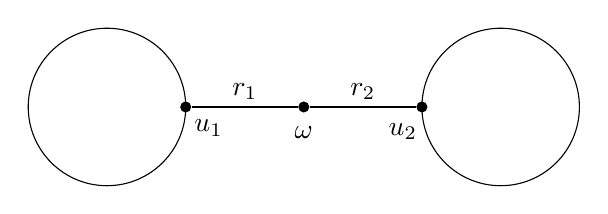
\begin{tikzpicture}[scale=1, every node/.style=fill,circle,minimum size=4pt,inner sep=0pt]
			\draw (0,0) circle (1);
			\draw (5,0) circle (1);
			\node[label={[label distance=3pt]320:{$u_1$}}] (u1) at (1,0) {};
			\node[label={[label distance=3pt]270:{$\omega$}}]  (omega) at (2.5,0) {};
			\node[label={[label distance=3pt]240:{$u_2$}}]  (u2) at (4,0) {};
			\draw (u1) -- (omega);
			\draw (omega) -- (u2);
			\node[fill=none] at (1.75,0.2) {$r_1$};
			\node[fill=none] at (3.25,0.2) {$r_2$};
		\end{tikzpicture}
		\subcaption{Verbindung der Teilnetzwerke über genau einen Knoten}
		\label{fig:1-1}
		\end{subfigure}
	\hfill
	\begin{subfigure}[t]{0.4\textwidth}
		\centering
			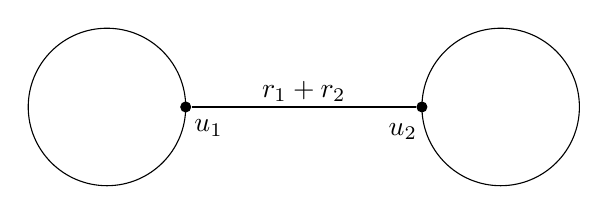
\begin{tikzpicture}[scale=1, every node/.style=fill,circle,minimum size=4pt,inner sep=0pt]
			\draw (0,0) circle (1);
			\draw (5,0) circle (1);
			\node[label={[label distance=3pt]320:{$u_1$}}] (u1) at (1,0) {};
			\node[label={[label distance=3pt]240:{$u_2$}}]  (u2) at (4,0) {};
			\draw (u1) -- (u2);
			\node[fill=none] at (2.5,0.2) {$r_1 + r_2$};
			\end{tikzpicture}	
		\subcaption{Ersetzen des Knotens durch Kante}
		\label{fig:1-2}
		\end{subfigure}
	\caption{Ersetzen von $\omega$}	
	\end{figure}


Wieso ist das nützlich?
\begin{beispiel}
	Sei $(X_n)_n$ die einfache Irrfahrt auf $\benb{0,n}$ mit Start in $k$. Frage: Was ist $\prop{\tau_0 < \tau_n}[][k]$? Wir wissen: Dies ist $v(k)$, wenn in $0$ eine Spannung $1$ und in $n$ eine Spannung $0$ anlegt.
	
	\begin{figure}[t]
		\begin{subfigure}[t]{0.4\textwidth}
			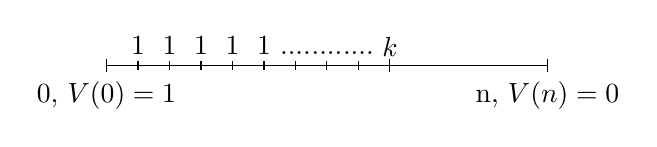
\begin{tikzpicture}[scale = 0.8]
				\draw(0,0) to (7,0);
				
				\draw(0,3pt) to (0,-3pt) node[below] {0, $V(0) = 1$};
				\draw(7,3pt) to (7,-3pt) node[below] {n, $V(n) = 0$};
				\foreach \x in {1,...,5}
				{
					\draw(0.5*\x,2pt) to (0.5*\x,-2pt) node[above=2pt] {1};
				}
				\foreach \x in {6,...,8}
				{
					\draw(0.5*\x,2pt) to (0.5*\x,-2pt) node[above=2pt] {....};
				}
				\draw(4.5,3pt) to (4.5,-3pt) node[above=2pt] {$k$};
			\end{tikzpicture}
			\subcaption{}
			\label{fig:1-3-1}
		\end{subfigure}
		\hfill
		\begin{subfigure}[t]{0.4\textwidth}
			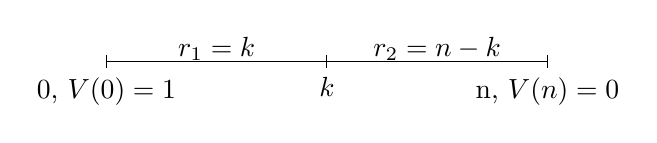
\begin{tikzpicture}[scale = 0.8]
			\draw(0,0) to (7,0);
			\draw(0,3pt) to (0,-3pt) node[below] {0, $V(0) = 1$};
			\draw(7,3pt) to (7,-3pt) node[below] {n, $V(n) = 0$};
			\draw(3.5,3pt) to (3.5,-3pt) node[below] {$k$};
			\node[fill=none] at (1.75,0.2) {$r_1 = k$};
			\node[fill=none] at (5.25,0.2) {$r_2 = n-k$};	
			\end{tikzpicture}
			\subcaption{}
			\label{fig:1-3-2}
		\end{subfigure}
		\caption{Zusammenführen mehrerer Kanten in Reihe}
	\end{figure}
	
	Nach dem Gesetz der Reihenschaltung kann man dieses Netzwerk (\ref{fig:1-3-1}) in folgendes Überführen(\ref{fig:1-3-2}) :
	\begin{gather}
		v(k) = \sum\limits_{y \sim k}\frac{c_{ky}}{\pi(k)}v_y = \frac{c_{k0}}{\pi(k)} \\
		\pi(k) = c_{k0} + c_{kn} = \frac{1}{k} + \frac{1}{k-n} = \frac{n}{k(n-k)} = \frac{n-k}{n}
	\end{gather}
	Allgemein gilt mit $q = 1-p$: $c(i,i+1) = \enb{\frac{p}{q}}^i$ und $v(i,i+1) = \enb{\frac{q}{p}}^i$.

	Dann kann man das Netzwerk (welches Analog zu \autoref{fig:1-3-2} ist) zusammenfassen mit 
	\begin{align}
		r_1 = \sum\limits_{i = 0}^{k-1}\enb{\frac{q}{p}}^i && r_1 = \sum\limits_{i = k}^{n-1}\enb{\frac{q}{p}}^i
	\end{align}

	Wieder ist 
	\begin{align}
		v_k = \frac{c_{k0}}{\pi(k)} && \pi(z) = \frac{\sum\limits_{i=0}^{n-1}\enb{\frac{q}{p}}^i}{\enb{\sum\limits_{i=0}^{k-1}\enb{\frac{q}{p}}^i} \enb{\sum\limits_{i=k}^{n-1} \enb{\frac{q}{p}}^i}} \\
	\end{align}
	\begin{align}
		\Rightarrow v_k = \frac{\sum\limits_{i=k}{n-1} \enb{\frac{q}{p}}^i}{\sum\limits_{i=0}^{n-1}\enb{\frac{q}{p}}^i} = \dots = \frac{\enb{\frac{p}{q}}^{n-k} -1}{\enb{\frac{p}{q}}^n-1}
 	\end{align}
\end{beispiel}
2. Prinzip: Parallelschaltung \\
Man kann zwei parallele Leitungen mit Kapazitäten (Leitfähigkeiten) $c_1$ und $c_2$ durch eine einzige mit Leitfähigkeit $c_1+c_2$ ersetzen. Mit anderen Worten: In \autoref{fig:1-4} lässt sich die Doppelkante $(u_1,u_2)$ mit Leitfähigkeit $c_1$ und $c_2$ durch eine Kante $c_1+c_2$ ersetzen, ohne dass sich an den Spannungen und Strömen im Restnetzwerk etwas ändert. Übung: Beweis.

\begin{figure}
	\centering
	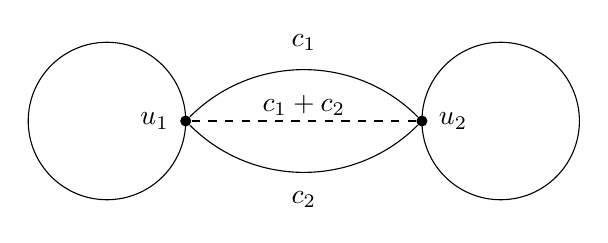
\begin{tikzpicture}[scale=1, every node/.style=fill,circle,minimum size=4pt,inner sep=0pt]
	\draw (0,0) circle (1);
	\draw (5,0) circle (1);
	\node[label={[label distance=3pt]180:{$u_1$}}] (u1) at (1,0) {};
	\node[label={[label distance=3pt]0:{$u_2$}}]  (u2) at (4,0) {};
	\draw [bend angle=45, bend right] (u1) to (u2);
	\draw [bend angle=45, bend left] (u1) to (u2);
	\node[fill=none] at (2.5,1) {$c_1$};
	\node[fill=none] at (2.5,-1) {$c_2$};
	\draw [dashed] (u1) to (u2);
	\node[fill=none] at (2.5,.2) {$c_1 + c_2$};
	\end{tikzpicture}	
	\caption{Zusammenlegen zweier parallel geschalteter Kanten.}
	\label{fig:1-4}
\end{figure}

\begin{beispiel} 
	Gefragt: $\propE{a \to z}$ im Netzwerk von \autoref{fig:1-5}. Durch die abgebildete Simplifizierung des Netwerkes erhalten wir direkt 
	\begin{align}
		\prop{a \to z} = \frac{\mathcal{C}(a \leftrightarrow z)}{i(a)} = \frac{\frac{7}{12}}{3} = \frac{7}{36}
	\end{align}
	%!TEX root = ../../WTG.tex

\begin{figure}
	\centering
	\subcaptionbox{Ausgangsnetzwerk}[0.49\textwidth]{
		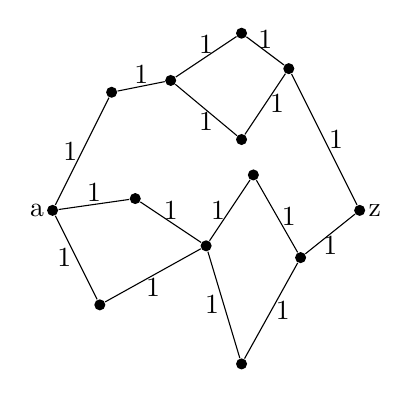
\begin{tikzpicture}[scale=1.5, every node/.style=fill,circle,minimum size=4pt,inner sep=0pt]
			\node [label=left:{a}] (a) at (0,0) {};
			\node (1) at (0.5,1) {};
			\node (2) at (1,1.1) {};
			\node (3) at (1.6,1.5) {};
			\node (4) at (1.6,0.6) {};
			\node (5) at (2,1.2) {};
			\node[label=right:{z}] (z) at (2.6,0) {}; 
			\node (6) at (0.7,0.1) {};
			\node (7) at (0.4,-0.8) {};
			\node (8) at (1.3,-0.3) {};
			\node (9) at (1.7,0.3) {};
			\node (10) at (1.6,-1.3) {};
			\node (11) at (2.1,-0.4) {};
			\draw (a) -- (1) node [midway, left, fill=none] {1};	
			\draw (1) -- (2) node [midway, above, fill=none] {1};	
			\draw (2) -- (3) node [midway, above, fill=none] {1};	
			\draw (2) -- (4) node [midway, below, fill=none] {1};
			\draw (4) -- (5) node [midway, right, fill=none] {1};		
			\draw (3) -- (5) node [midway, above, fill=none] {1};	
			\draw (5) -- (z) node [midway, right, fill=none] {1};	
			\draw (a) -- (6) node [midway, above, fill=none] {1};
			\draw (a) -- (7) node [midway, left, fill=none] {1};
			\draw (6) -- (8) node [midway, above, fill=none] {1};
			\draw (7) -- (8) node [midway, below, fill=none] {1};	
			\draw (8) -- (9) node [midway, left, fill=none] {1};	
			\draw (8) -- (10) node [midway, left, fill=none] {1};
			\draw (9) -- (11) node [midway, right, fill=none] {1};	
			\draw (10) -- (11) node [midway, right, fill=none] {1};	
			\draw (11) -- (z) node [midway, below, fill=none] {1};						
			%\draw (d) -- \node at (1,1) {} \node[fill=none,midway,label=above:{1}] {};
		\end{tikzpicture}
	}
	\hfill
	\subcaptionbox{Reihenschaltungen zusammengezogen}[0.49\textwidth]{
		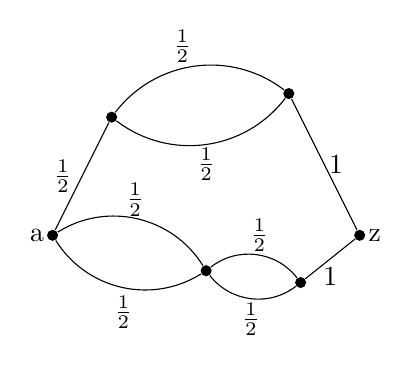
\begin{tikzpicture}[scale=1.5, every node/.style=fill,circle,minimum size=4pt,inner sep=0pt]
		\node [label=left:{a}] (a) at (0,0) {};
		\node (1) at (0.5,1) {};
		\node (2) at (2,1.2) {};
		\node[label=right:{z}] (z) at (2.6,0) {}; 
		\node (3) at (1.3,-0.3) {};
		\node (4) at (2.1,-0.4) {};
		
		\draw (a) -- (1) node [midway, left, fill=none] {$\frac{1}{2}$};
		\draw[bend angle=45,bend left] (1) to (2);
		\node [fill=none] at (1.1,1.6) {$\frac{1}{2}$};
		\draw[bend angle=45,bend right] (1) to (2);
		\node [fill=none] at(1.3,0.6) {$\frac{1}{2}$};
		\draw (2) -- (z) node [midway, right, fill=none] {$1$};
		\draw[bend angle=45,bend left] (a) to (3);
		\node [fill=none] at (0.7,0.3){$\frac{1}{2}$};
		\draw[bend angle=45,bend right] (a) to (3);
		\node [fill=none] at(0.6,-0.65) {$\frac{1}{2}$};	
		\draw[bend angle=45,bend left] (3) to (4);
		\node [fill=none] at (1.75,0) {$\frac{1}{2}$};
		\draw[bend angle=45,bend right] (3) to (4);
		\node [fill=none] at (1.68,-0.71) {$\frac{1}{2}$};	
		\draw (4) -- (z) node [midway, below=2pt, fill=none] {$1$};				
		%\draw (d) -- \node at (1,1) {} \node[fill=none,midway,label=above:{1}] {};
		\end{tikzpicture}
	}
	\hfill
	\subcaptionbox{Parallelschaltungen zusammengezogen}[0.30\textwidth]{
		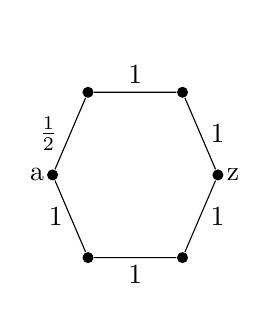
\begin{tikzpicture}[scale=1.5, every node/.style=fill,circle,minimum size=4pt,inner sep=0pt]
			\node [label=left:{a}] (a) at (0,0) {};
			\node (1) at (0.3,0.7) {};
			\node (2) at (1.1,0.7) {};
			\node[label=right:{z}] (z) at (1.4,0) {}; 
			\node (3) at (0.3,-0.7) {};
			\node (4) at (1.1,-0.7) {};
			\draw (a) -- (1) node [midway, left=1pt, fill=none] {$\frac{1}{2}$};
			\draw (1) -- (2) node [midway, above=2pt, fill=none] {$1$};
			\draw (2) -- (z) node [midway, right=2pt, fill=none] {$1$};
			\draw (a) -- (3) node [midway, left=1pt, fill=none] {$1$};
			\draw (3) -- (4) node [midway, below=2pt, fill=none] {$1$};
			\draw (4) -- (z) node [midway, right=2pt, fill=none] {$1$};
			\node[fill=none] at (0,-0.8) {}; 
			\node[fill=none] at (0,1.2) {};	
		\end{tikzpicture}
	}
	\hfill
	\subcaptionbox{Reihenschaltungen erneut zusammengezogen}[0.30\textwidth]{
		\begin{tikzpicture}[scale=1.5, every node/.style=fill,circle,minimum size=4pt,inner sep=0pt]
			\node [label=left:{a}] (a) at (0,0) {};
			\node[label=right:{z}] (z) at (1.4,0) {}; 
			\draw[bend angle=45,bend right] (a) to (z);
			\node [fill=none] at (0.7,0.5) {$\frac{1}{4}$};
			\draw[bend angle=45,bend left] (a) to (z);
			\node [fill=none] at (0.7,-0.5) {$\frac{1}{3}$};
			\node[fill=none] at (0,-0.8) {}; 
			\node[fill=none] at (0,1.2) {};
		\end{tikzpicture}
	}
	\hfill
	\subcaptionbox{Parallelschaltungen erneut zusammengezogen}[0.30\textwidth]{
		\begin{tikzpicture}[scale=1.5, every node/.style=fill,circle,minimum size=4pt,inner sep=0pt]
		\node [label=left:{a}] (a) at (0,0) {};
		\node[label=right:{z}] (z) at (1.4,0) {}; 
		\node[fill=none] at (0,-0.8) {}; 
		\node[fill=none] at (0,1.2) {};
		\draw (a) to (z);
		\node [fill=none] at (0.7,0.2) {$\frac{7}{12}$};
		\end{tikzpicture}	
	}
	\caption{Schritt für Schritt Simplifizierung eines Netzwerks}
	\label{fig:1-5}
\end{figure}
\end{beispiel}


\begin{beispiel}
	Gesucht $\prop{a \to z}$ im Netzwerk von \autoref{fig:1-6}. Hier wenden wir ein \enquote{Physikerargument} an:
	Die Situation von $b$ und $c$ ist vollkommen identisch, daher gilt $v(b) = v(c)$ und somit $i(b,c) = 0$. Also kann man die Kante, welche die beiden verbindet auch einfach weglassen. Danach vereinfacht man das Netzwerk schrittweise analog zum vorigen Beispiel und erhält so
	\begin{align}
		\mathcal{C}(a \leftrightarrow z) = \frac{2}{3} \Rightarrow \prop{a \rightarrow z} = \frac{\frac{2}{3}}{2}= \frac{1}{3}
	\end{align}
	Spätestens wenn aber die an $b$ und $c$ angrenzenden Kanten unterschiedliches Gewicht haben wird das Argument allerdings problematisch.
	\begin{figure}
		\centering
		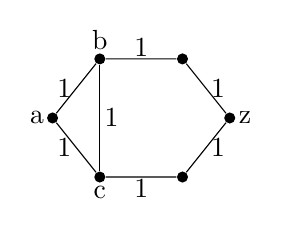
\begin{tikzpicture}[scale=1.5, every node/.style=fill,circle,minimum size=4pt,inner sep=0pt]
		
			\node [label=left:{a}] (a) at (0,0) {};
			\node [label=above:{b}] (1) at (0.4,0.5) {};
			\node (2) at (1.1,0.5) {};
			\node [label=below:{c}](3) at (0.4,-0.5) {};
			\node (4) at (1.1,-0.5) {};
			\node[label=right:{z}] (z) at (1.5,0) {}; 
			
			\draw (a) -- (1) node [midway, left, fill=none] {1};	
			\draw (1) -- (2) node [midway, above, fill=none] {1};	
			\draw (2) -- (z) node [midway, right, fill=none] {1};	
			\draw (a) -- (3) node [midway, left, fill=none] {1};
			\draw (3) -- (4) node [midway, below, fill=none] {1};	
			\draw (4) -- (z) node [midway, right, fill=none] {1};	
			\draw (1) -- (3) node [midway, right, fill=none] {1};
			
		\end{tikzpicture}
		\caption{Ausgangsnetzwerk für \enquote{Physikertrick}}
		\label{fig:1-6}
	\end{figure}
\end{beispiel}

\subsubsection*{3. Prinzip: Y--$\Delta$--Prinzip}
Auch Stein--Dreieck--Prinzip genannt. Netzwerke in denen man eine der Konfigurationen aus \autoref{fig:1-7} durch die andere ersetzt, sind äquivalent, falls 

\begin{figure}
	\centering
	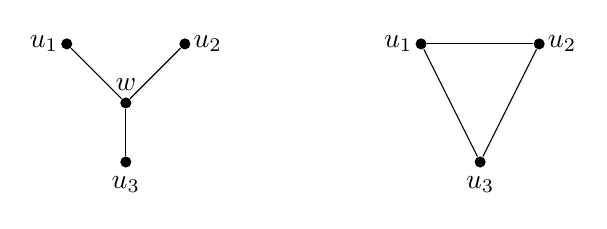
\begin{tikzpicture}[scale=1.5, every node/.style=fill,circle,minimum size=4pt,inner sep=0pt]
		\node [label=left:{$u_1$}] (u1) at (-0.5,0.5) {};
		\node [label=right:{$u_2$}] (u2) at (0.5,0.5) {};
		\node [label=below:{$u_3$}] (u3) at (0,-0.5) {};
		\node [label=above:{$w$}] (w) at (0,0) {};
		
		\node [label=left:{$u_1$}] (u1d) at (2.5,0.5) {};
		\node [label=right:{$u_2$}] (u2d) at (3.5,0.5) {};
		\node [label=below:{$u_3$}] (u3d) at (3,-0.5) {};
		
		\draw (u1) -- (w);
		\draw (u2) -- (w);
		\draw (u3) -- (w);
		\draw (u1d) -- (u2d);
		\draw (u2d) -- (u3d);
		\draw (u3d) -- (u1d);		 
	\end{tikzpicture}
	\caption{Äquivalente Konfigurationen}
	\label{fig:1-7}
\end{figure}


\begin{align}
	c(w, u_i) \cdot c(u_{i-1},u_{i+1}) = \gamma, \quad \forall i\ \text{mod}\ 3 &&
	\text{mit }\quad \gamma  = \frac{\prod_{i} c(w,u_i)}{\sum_{i}c(w,u_i)}
\end{align}
\subsubsection*{4. Prinzip (trivial):}
Man kann Knoten von Grad 1 hinzufügen oder entfernen. Selbiges Gilt für Schlaufen.

\newpage



